\chapter[APÊNDICE \ref{Ap:Cavity3}]{Análise do problema de cavidade bidimensional em diferentes modelos}
\label{Ap:Cavity3}

O seguinte exemplo busca verificar a necessidade da utilização do modelo de turbulência em simulações de malha menos refinada em situação de número de Reynolds elevado. Para isso assumiu-se um problema com $\Rey=10000$, sendo o domínio computacional gerado pela divisão de cada aresta em 20 segmentos, totalizando, assim, 800 elementos finitos triangulares, dispostos de forma estruturada com orientação à esquerda. As simulações foram conduzidas sem a utilização de nenhum modelo de turbulência, seguido dos modelos LES e VMS. Para cada uma das simulações empregou-se elementos de aproximação linear, quadrática e Taylor-Hood P2P1, sendo que para os dois primeiros aplicou-se um estabilizador PSPG, uma vez que esses elementos não possuem estabilidade no campo de pressões. Assim, chegou-se em 441 nós e 1323 DOF para a simulação contendo elementos lineares, 1681 nós e 5043 DOF para quadráticos e 1681 nós e 3803 DOF para P2P1. A simulação foi mantida em um intervalo de tempo $t\in[0,500]$, discretizado em $\Delta t=0,1$, sendo que a condição inicial foi de $\BB{u}=\BB{0}$ em todos os pontos no interior do domínio. A Tabela \ref{tab:comp-res2} apresenta de forma qualitativa os resultados obtidos. O campo de velocidades obtidos para cada simulação no instante $t=500$ é apresentado na Figura \ref{fig:cavity-coarse}.

\begin{table}[h!]
    \centering
    \caption{Comparação dos resultados apresentados em simulação em modelo, com aplicação de LES e de VMS.}
    \begin{tabularx}{\textwidth}{|p{2cm}|p{3cm}|X|}
        \hline
        Tipo de elemento      & Simulação  & Resultado                                                         \\\hline
        \MR{3}{*}{Linear}     & Sem modelo & Sem sentido físico                                                \\\cline{2-3}
                              & LES        & Formação de vórtice com valores espúrios próximos à face superior \\\cline{2-3}
                              & VMS        & Formação de vórtice com variação pequena do campo de velocidades  \\\hline
        \MR{3}{*}{Quadrático} & Sem modelo & Não houve avanço na solução (se manteve na condição inicial)      \\\cline{2-3}
                              & LES        & Formação de vórtice                                               \\\cline{2-3}
                              & VMS        & Formação de vórtice                                               \\\hline
        \MR{3}{*}{P2P1}       & Sem modelo & Divergência                                                       \\\cline{2-3}
                              & LES        & Não atingiu o regime permanente                                   \\\cline{2-3}
                              & VMS        & Formação de vórtice                                               \\\hline
    \end{tabularx}
    \\Fonte: Presente trabalho (\the\year).
    \label{tab:comp-res2}
\end{table}

\begin{figure}[h!]
    \centering
    \caption{Campos de velocidades no instante $t=100$.}
    \begin{subfigure}{\textwidth}\centering
        \begin{subfigure}{\textwidth}\centering
            \begin{subfigure}{.32\textwidth}
                \caption*{\textbf{Elemento Linear.}}
                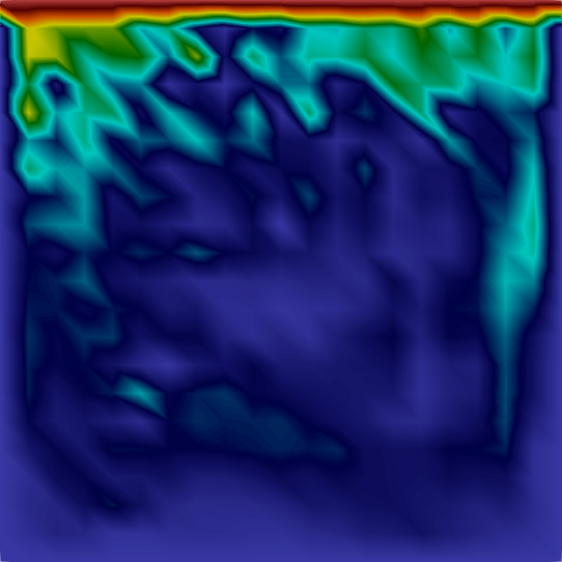
\includegraphics[width=\linewidth]{Figuras/cavity-poor/None-Lin.png}
            \end{subfigure}
            \begin{subfigure}{.32\textwidth}
                \caption*{\textbf{Elemento quadrático.}}
                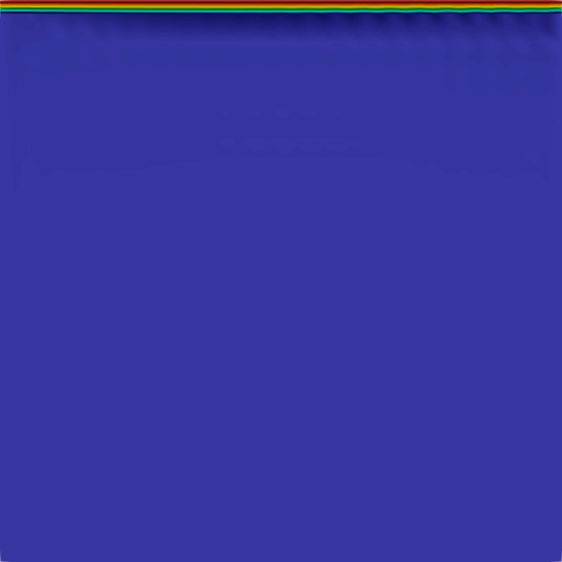
\includegraphics[width=\linewidth]{Figuras/cavity-poor/None-Qua.png}
            \end{subfigure}
            \begin{subfigure}{.32\textwidth}
                \caption*{\textbf{Elemento P2P1.}}
                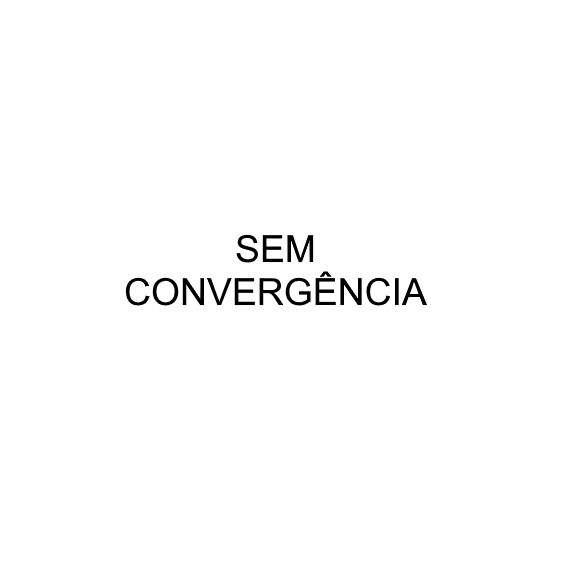
\includegraphics[width=\linewidth]{Figuras/cavity-poor/None-TH.png}
            \end{subfigure}
            \caption{Simulação sem modelo.}
        \end{subfigure}
        \begin{subfigure}{\textwidth}\centering
            \begin{subfigure}{.32\textwidth}
                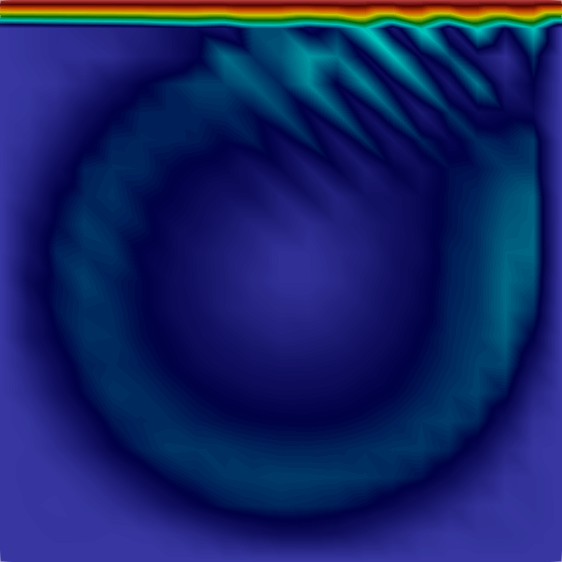
\includegraphics[width=\linewidth]{Figuras/cavity-poor/LES-Lin.png}
            \end{subfigure}
            \begin{subfigure}{.32\textwidth}
                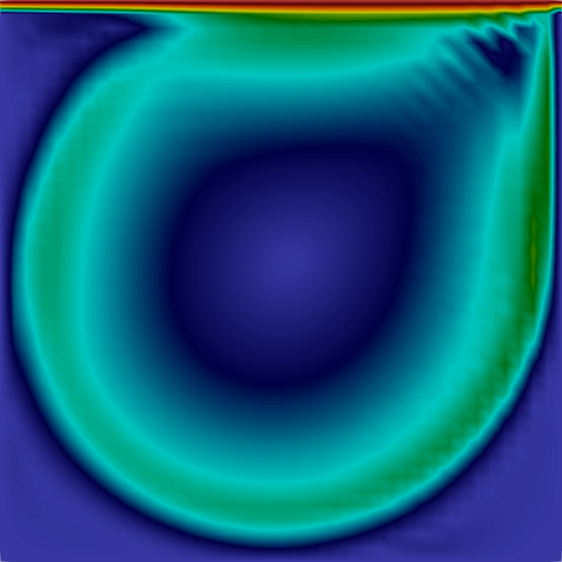
\includegraphics[width=\linewidth]{Figuras/cavity-poor/LES-Qua.png}
            \end{subfigure}
            \begin{subfigure}{.32\textwidth}
                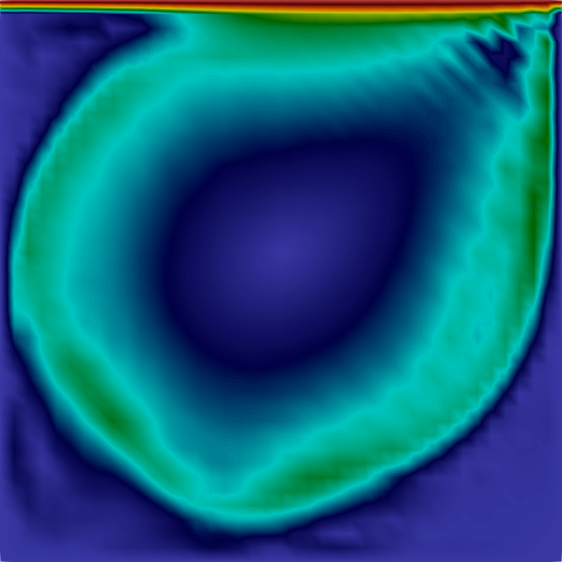
\includegraphics[width=\linewidth]{Figuras/cavity-poor/LES-TH.png}
            \end{subfigure}
            \caption{Simulação LES.}
        \end{subfigure}
        \begin{subfigure}{\textwidth}\centering
            \begin{subfigure}{.32\textwidth}
                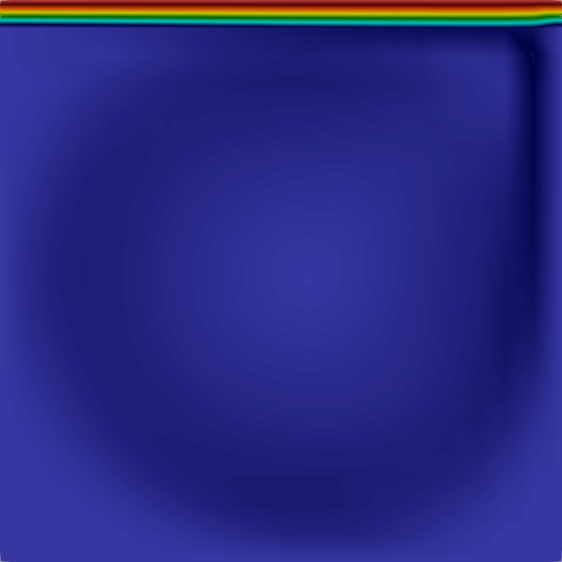
\includegraphics[width=\linewidth]{Figuras/cavity-poor/VMS-Lin.png}
            \end{subfigure}
            \begin{subfigure}{.32\textwidth}
                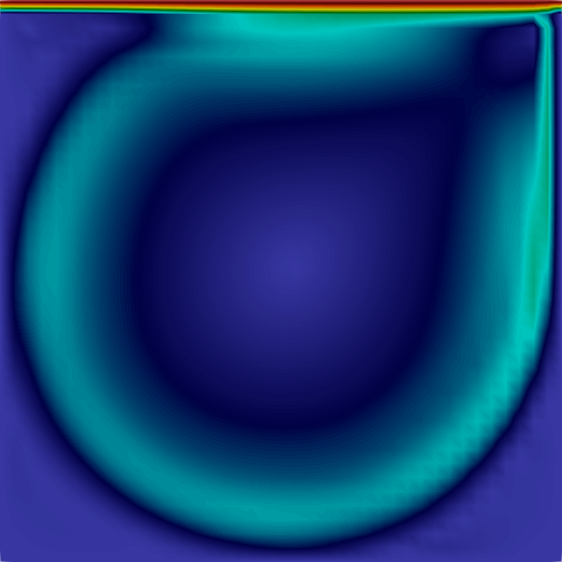
\includegraphics[width=\linewidth]{Figuras/cavity-poor/VMS-Qua.png}
            \end{subfigure}
            \begin{subfigure}{.32\textwidth}
                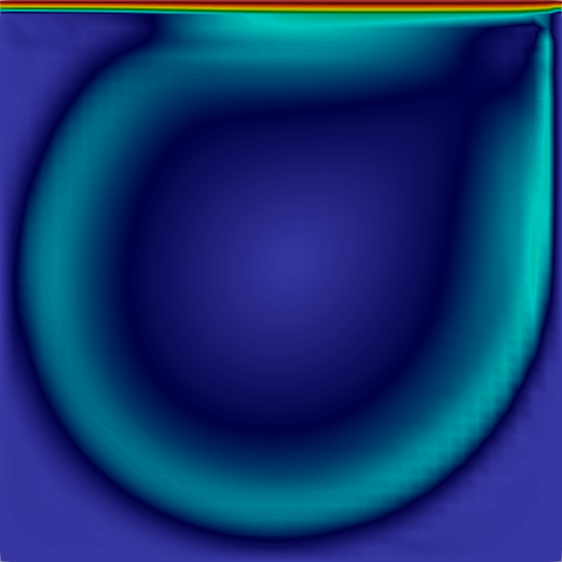
\includegraphics[width=\linewidth]{Figuras/cavity-poor/VMS-TH.png}
            \end{subfigure}
            \caption{Simulação VMS.}
        \end{subfigure}
        \begin{subfigure}{.5\textwidth}\centering
            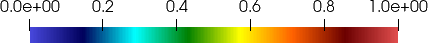
\includegraphics[width=\linewidth]{Figuras/cavity-poor/legenda.png}
        \end{subfigure}
    \end{subfigure}
    \label{fig:cavity-coarse}
    \\Fonte: Presente trabalho (\the\year).
\end{figure}

Logo, verifica-se que as simulações sem a aplicação de modelos de turbulência não foram capazes de simular o comportamento do escoamento. Por outro lado, mesmo em uma situação de malha grosseira, as simulações empregando LES e VMS foram capazes de capturar esse comportamento. No entanto a simulação modelada por LES em elemento P2P1 não atingiu o regime permanente.